\begin{frame}{Hyperparameter Sensitivity}

Let $\epsilon$ be a real-valued hyperparameter for the stick-breaking distribution
(e.\ g., this could be the $\alpha$ concentration parameter, or it could parameterize a functional shape).

\pause

{\bf Main idea: } We approximate the dependence of $\eta^*$ on $\epsilon$ with a first-order
Taylor expansion:

\begin{align*}
  \eta^*(\epsilon)  &\approx  \eta^*(0) +
  \frac{d \eta^*(\epsilon)}{d\epsilon^T}\Big|_{\epsilon=0} \epsilon
\end{align*}

\pause

Notes:
\begin{itemize}
\item Evaluation of the derivative can be done efficiently using formulas from
{\color{blue} \href{https://arxiv.org/abs/1709.02536}{Giordano et al. 2018}}
and modern
{\color{blue} \href{https://jax.readthedocs.io/en/latest/}{automatic differentiation tools}}.

\item We only use a linear approximation for the map $\epsilon \mapsto \eta^*(\epsilon)$. We retain nonlinearities in the map $\eta^* \mapsto
\Expect_{q_{\eta^*}} \left[ \#\text{clusters} \right]$.

\end{itemize}
\end{frame}

\begin{frame}{A simple example: iris data}

We fit a Gaussian mixture model with a DP prior to
the iris data.

\begin{figure}[!h]
  \centering
  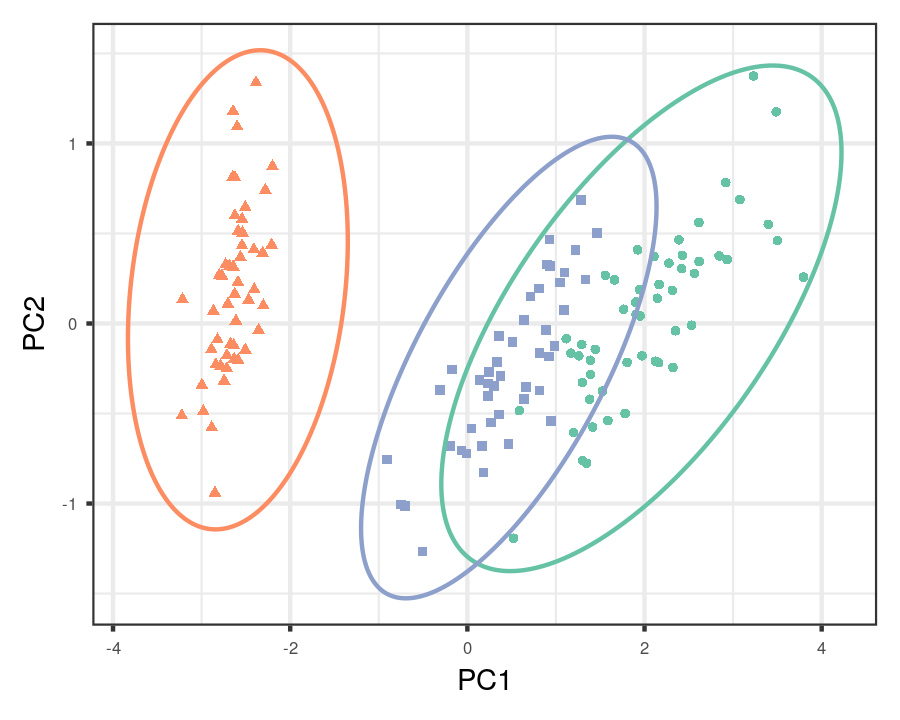
\includegraphics[width = 0.6\textwidth]{./figures/iris_init_fit.png}
  \caption*{The iris data in principal component space and GMM fit at $\alpha = 6$.}
\end{figure}

\end{frame}

\begin{frame}{iris data: parametric sensitivity}

\begin{figure}[!h]
  \only<1>{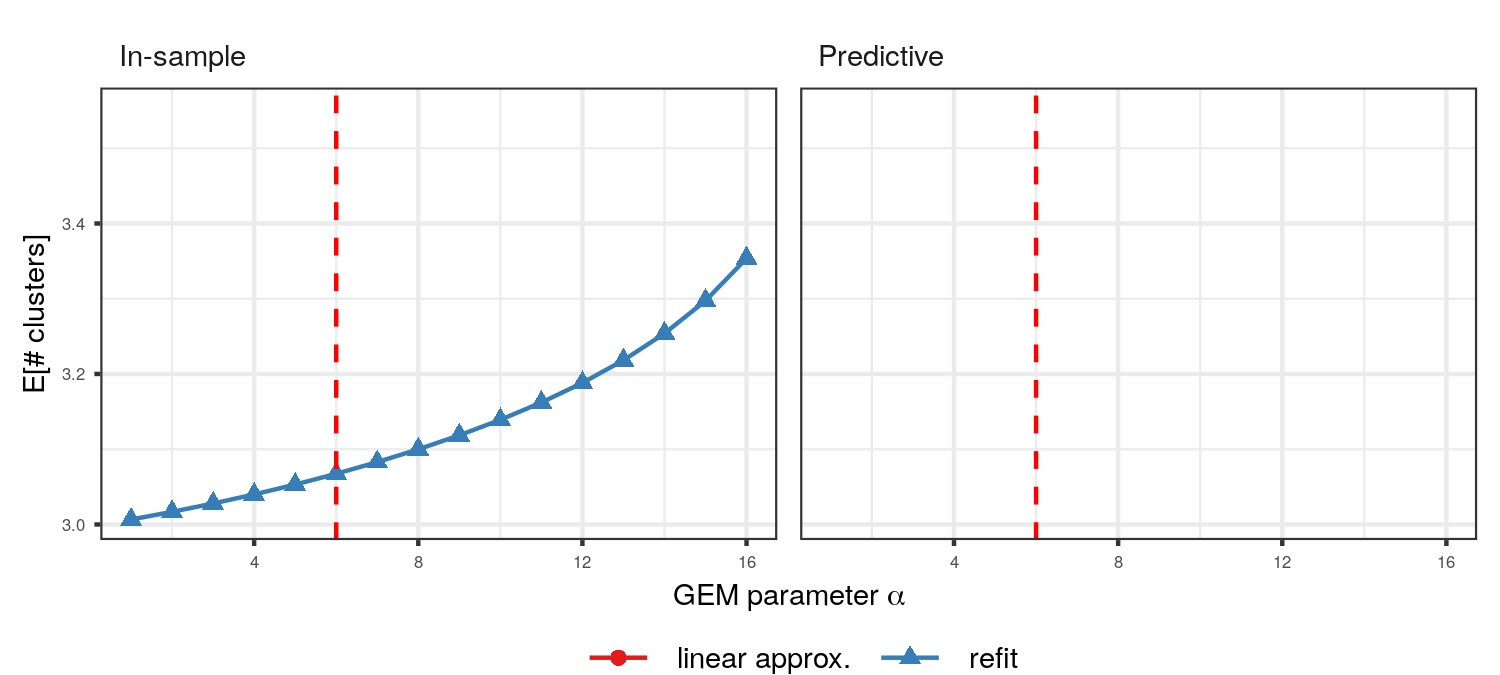
\includegraphics[width = \textwidth]{./figures/iris_alpha_sens0.png}}%
  \only<2>{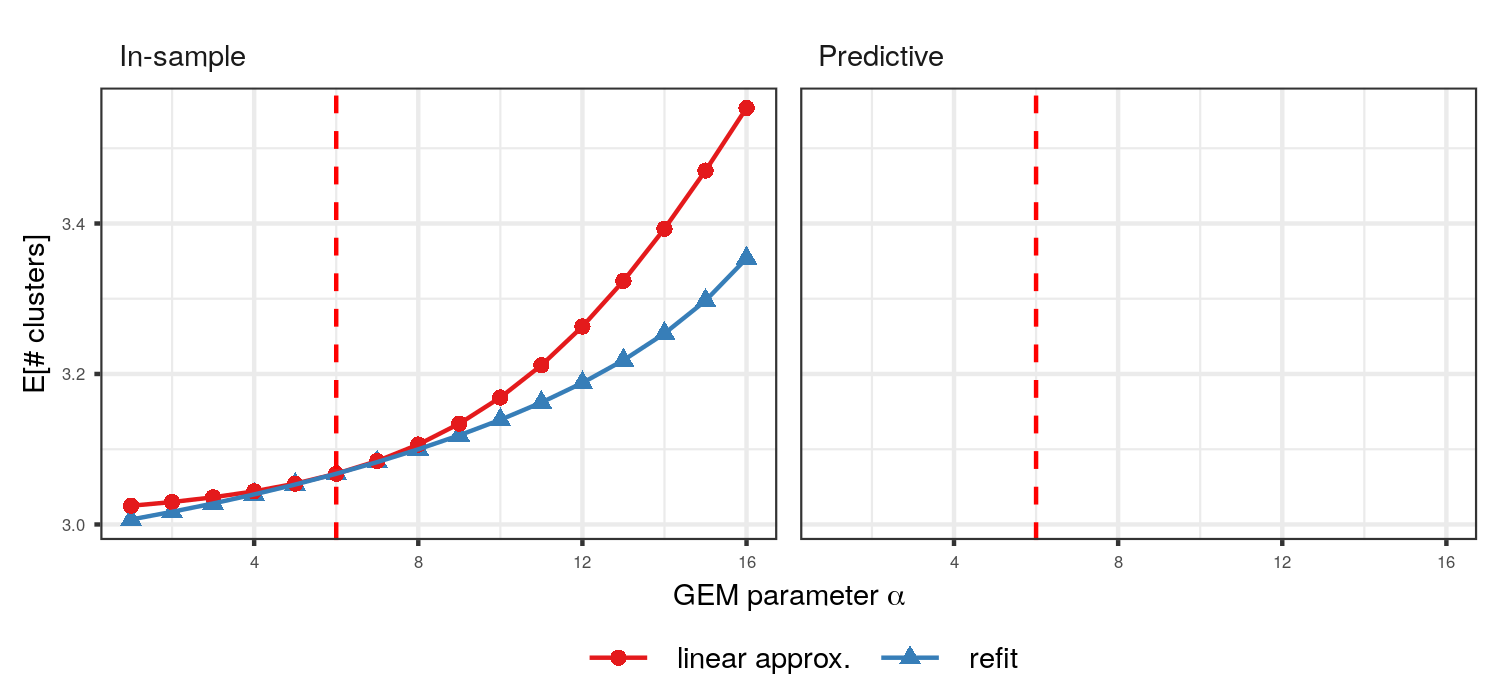
\includegraphics[width = \textwidth]{./figures/iris_alpha_sens1.png}}%
  \only<3>{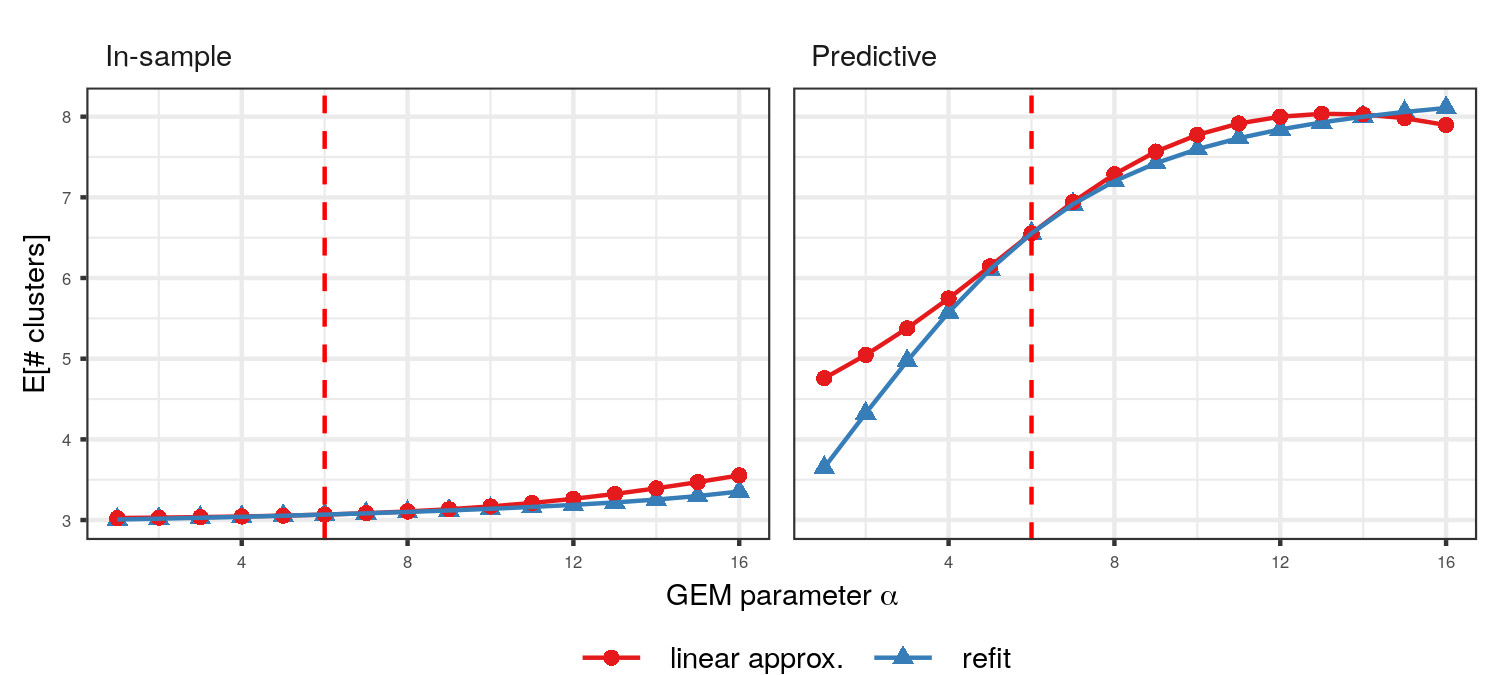
\includegraphics[width = \textwidth]{./figures/iris_alpha_sens2.png}}
  \caption*{The expected number of posterior clusters in the iris data as $\alpha$ varies.}
\end{figure}

\end{frame}
